% !TEX root = ../CourseOT.tex


%%%%%%%%%%%%%%%%%%%%%%%%%%%%%%%%%%%%%%%%%%%%%%%%%%%%%%%%%%%%%%%%%%%%%%%%%%%
%%%%%%%%%%%%%%%%%%%%%%%%%%%%%%%%%%%%%%%%%%%%%%%%%%%%%%%%%%%%%%%%%%%%%%%%%%%
%%%%%%%%%%%%%%%%%%%%%%%%%%%%%%%%%%%%%%%%%%%%%%%%%%%%%%%%%%%%%%%%%%%%%%%%%%%
\section{Sinkhorn}

%%%%%%%%%%%%%%%%%%%%%%%%%%%%%%%%%%%%%%%%%%%%%%%%%%%%%%%%%%%%%%%%%%%%%%%%%%%
\subsection{Entropic Regularization for Discrete Measures}


%%%%%
\paragraph{Relative entropy}

The Kullback-Leibler divergence is defined as
\eql{\label{eq-kl-defn}
	\KLD(\P|\Q) \eqdef \sum_{i,j}  \P_{i,j} \log\pa{\frac{\P_{i,j}}{\Q_{i,j}}} - \P_{i,j} + \Q_{i,j}.
}
with the convention $0\log(0)=0$ and $\KLD(\P|\Q)=+\infty$ if there exists some $(i,j)$ such that $\Q_{i,j}=0$ but $\P_{i,j} \neq 0$. 
%
The special case $\KLD(\P|\ones)$ corresponds to minus the Shannon-Boltzmann entropy. 
%
The function $\KLD(\cdot|\Q)$ is strongly convex, because its hessian is $\partial^2 \KLD(\P|\Q)=\diag(1/\P_{i,j})$ and $\P_{i,j} \leq 1$. 
%
Note that since in what follows $\P$ and $\Q$ are actually probability distributions, one has $\KLD(\P|\Q) \eqdef \sum_{i,j}  \P_{i,j} \log\pa{\frac{\P_{i,j}}{\Q_{i,j}}}$, but considering the extra terms gives cleaner expressions, in particular $\nabla \KLD(\P|\Q) = \log(\P/\Q)$ and duality formula reads more nicely. And for later, it will be important to have this normalization when considering unbalanced OT (see Section~\ref{sec-unbalanced}).

$\KL$ is a particular instance (and actually the unique case) of both a $\phi$-divergence (as defined in Section~\ref{sec-phi-div}) and a Bregman divergence. This unique property is at the heart of the fact that this regularization leads to elegant algorithms and a tractable mathematical analysis. One thus has $\KLD(\P|\Q) \geq 0$ and  $\KLD(\P|\Q)=0$ if and only if $\P=\Q$ (see Proposition~\ref{phi-div-positive}).


%%%%%
\paragraph{Entropic Regularization for Discrete Measures.}

The idea of the entropic regularization of optimal transport is to use $\KLD$ as a regularizing function to obtain approximate solutions to the original transport problem~\eqref{eq-mk-discr}:
\eql{\label{eq-regularized-discr}
	\MKD_\C^\epsilon(\a,\b) \eqdef 
	\umin{\P \in \CouplingsD(\a,\b)}
		\dotp{\P}{\C} + \epsilon \KLD(\P|\a \otimes \b). 
} 
Here we used as a reference measure for the relative entropy $\a \otimes \b = (\a_i \b_j)_{i,j}$.
%
This choice of normalization, specially in this discrete setting, has no importance for the selection of the optimal $\P$ since it only affects the objective by a constant, as shown in the following proposition.

\begin{prop} For $\P \in \CouplingsD(\a,\b)$, one has
\eq{
	\KLD(\P|\a \otimes \b) = 
	\KLD(\P|\a' \otimes \b') - \KLD(\a|\a') - \KL(\b|\b').
} 
\end{prop}

\begin{proof}
This follows from 
\eq{
	\sum_{i,j} \P_{i,j} \log\frac{\P_{i,j}}{\a_i\b_j}
	= 
	\sum_{i,j} \P_{i,j} \log\frac{\P_{i,j}}{\a_i'\b_j'}
	+ 
	\sum_{i,j} \P_{i,j} \pa{\log\frac{\a_i'}{\a_i} + \log\frac{\b_j'}{\b_j}}.
} 
\end{proof}

This choice of normalization is however important to deal with situation where the support of $\a$ and $\b$ can change, and in particular when later we will deal with possibly continuous distribution. It also affect the values of the cost $\MKD_\C^\epsilon(\a,\b)$ and this normalization will be instrumental to define a proper Sinkhorn divergence. 


% Figure~\ref{fig-impact-eps} illustrates the effect of the entropy to regularize a linear program over the simples $\simplex_3$ (which can thus be visualized as a triangle in 2-D). Note how the entropy pushes the original LP solution away from the boundary of the triangle. The optimal $\P_\epsilon$ progressively moves toward an ``entropic center'' of the triangle. This is further detailed in the proposition below. The convergence of the solution of that regularized problem towards an optimal solution of the original linear program has been studied by~\cite{CominettiAsympt}.


%\begin{figure}
%\centering
%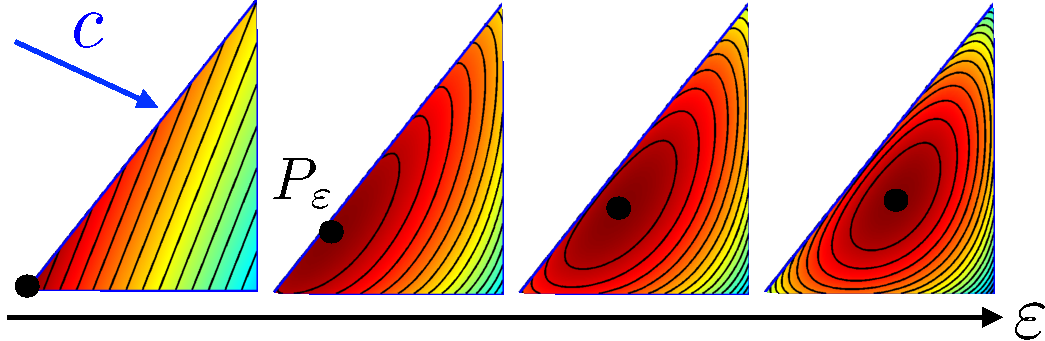
\includegraphics[width=.5\linewidth]{entropic/simplex}
%\caption{\label{fig-impact-eps}
%Impact of $\epsilon$ on the optimization of a linear function on the simplex, solving $\P_\epsilon = \argmin_{\P \in \simplex_3} \dotp{\C}{\P}-\epsilon\HD(\P)$ for a varying $\epsilon$. 
%}
%\end{figure}


%%%%%
\paragraph{Smoothing effect.}

Since the objective is a $\epsilon$-strongly convex function, problem~\ref{eq-regularized-discr} has a unique optimal solution. 
%
As studied in Section~\ref{}, this smoothing, beyond providing uniqueness, actually leads to $\MKD_\C^\epsilon(\a,\b)$ being a smooth function of $\a, \b$ and $\C$. 
%
The effect of the entropy is to act as a barrier function for the positivity constraint. As we will show next, this forces the solution $\P$ to be strictly positive on the support of $\a \otimes \b$. 

One has the following convergence property.
 
 
\begin{prop}[Convergence with $\epsilon$]\label{prop-convergence-eps}
The unique solution $\P_\epsilon$ of~\eqref{eq-regularized-discr} converges to the optimal solution with maximal entropy within the set of all optimal solutions of the Kantorovich problem, namely
\eql{\label{eq-entropy-conv-1}
	\P_\epsilon \overset{\epsilon \rightarrow 0}{\longrightarrow}
	\uargmin{\P} \enscond{ \KLD(\P|\a \otimes \b) }{
		\P \in \CouplingsD(\a,\b), \dotp{\P}{\C} = \MKD_\C(\a,\b)
	}
}
so that in particular
\eq{
	\MKD_\C^\epsilon(\a,\b) \overset{\epsilon \rightarrow 0}{\longrightarrow} \MKD_\C(\a,\b).
}
One has
\eql{\label{eq-entropy-conv-2}
	\P_\epsilon \overset{\epsilon \rightarrow \infty}{\longrightarrow}
	\a \otimes \b.
}
\end{prop}

\begin{proof}
	\textbf{Case $\epsilon \rightarrow 0$.}
	 We consider a sequence $(\epsilon_\ell)_\ell$ such that $\epsilon_\ell \rightarrow 0$ and $\epsilon_\ell > 0$.	
 	We denote $\P_\ell$ the solution of~\eqref{eq-regularized-discr} for $\epsilon=\epsilon_\ell$. 
	%
	Since $\CouplingsD(\a,\b)$ is bounded, we can extract a sequence (that we do not relabel for sake of simplicity) such that $\P_\ell \rightarrow \P^\star$. Since $\CouplingsD(\a,\b)$ is closed, $\P^\star \in \CouplingsD(\a,\b)$. We consider any $\P$ such that $\dotp{\C}{\P} = \MKD_\C(\a,\b)$. By optimality of $\P$ and $\P_\ell$ for their respective optimization problems (for $\epsilon=0$ and $\epsilon=\epsilon_\ell$), one has
 	\eql{\label{eq-proof-gamma-conv}
 		0 \leq \dotp{\C}{\P_\ell} - \dotp{\C}{\P} \leq \epsilon_\ell ( \KLD(\P_\ell|\a \otimes \b)-\KLD(\P|\a \otimes \b) ).
 	}
 	Since $\HD$ is continuous, taking the limit $\ell \rightarrow +\infty$ in this expression shows that 
 	$\dotp{\C}{\P^\star} = \dotp{\C}{\P}$ so that $\P^\star$ is a feasible point of~\eqref{eq-entropy-conv-1}. Furthermore, dividing by $\epsilon_\ell$ in~\eqref{eq-proof-gamma-conv} and taking the limit shows that 
 	$\KLD(\P|\a \otimes \b) \leq \KLD(\P^\star|\a \otimes \b)$, which shows that $\P^\star$ is a solution of~\eqref{eq-entropy-conv-1}. Since the solution $\P_0^\star$ to this program is unique by strict convexity of $\KL(\cdot|\a \otimes \b)$, one has $\P^\star = \P_0^\star$, and the whole sequence is converging. 
	
	
	\textbf{Case $\epsilon \rightarrow +\infty$.} Evaluating at $\a \otimes \b$ the energy, one has
	\eq{
		\dotp{\C}{\P_\epsilon} + \epsilon \KL(\P_\epsilon|\al \otimes \be) \leq \dotp{\C}{\al \otimes \be} + \epsilon \times 0
	}
	and since $\dotp{\C}{\P_\epsilon} \geq 0$, this leads to
	\eq{
		\KL(\P_\epsilon|\al \otimes \be) \leq \epsilon^{-1} \dotp{\C}{\al \otimes \be} \leq \frac{\norm{\C}_\infty}{\epsilon}
	}
	so that $\KL(\P_\epsilon|\al \otimes \be) \rightarrow 0$ and thus $\P_\epsilon \rightarrow \al \otimes \be$ since $\KL$ is a valid divergence.
\end{proof}


%\begin{figure}
%\centering
%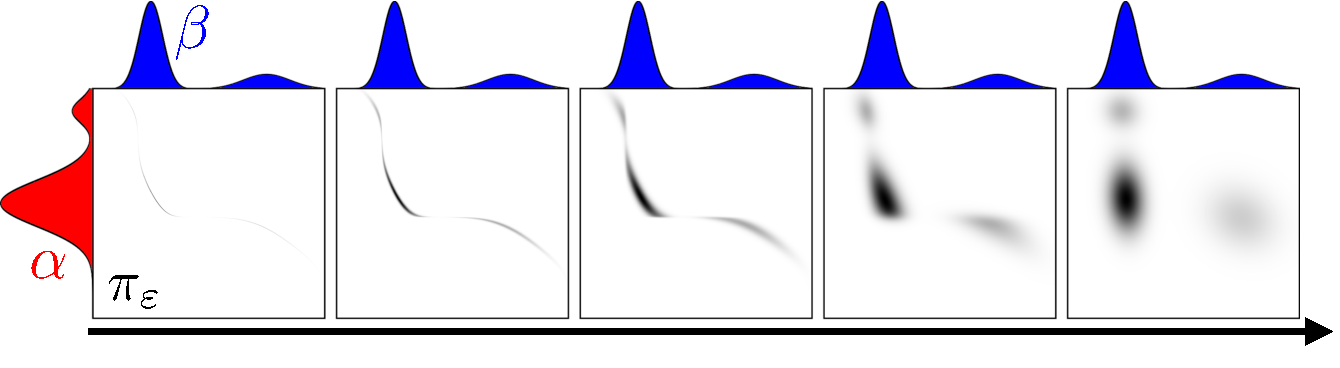
\includegraphics[width=.48\linewidth]{entropic/densities}
%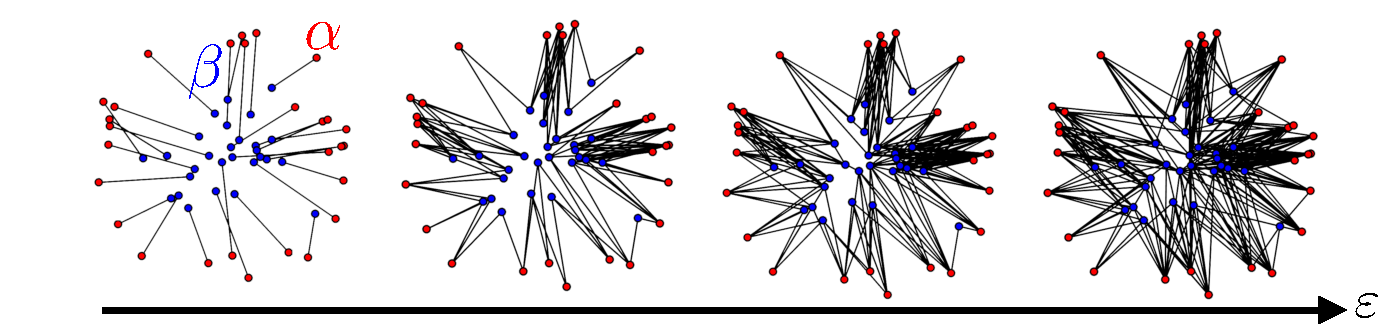
\includegraphics[width=.48\linewidth]{entropic/matching-2d}
%\caption{\label{fig-entropic}
%Impact of $\epsilon$ on coupling between densities and discrete distributions, illustrating Proposition~\ref{prop-convergence-eps}.
%%
%Left: between two 1-D densities. Right: between two 2-D discrete empirical densities with same number $n=m$ of points (only entries of the optimal $(\P_{i,j})_{i,j}$ above a small threshold are displayed as segments between $x_i$ and $y_j$).
%}
%\end{figure}




% \todo{First order expansion}


%%%%%%%%%%%%%%%%%%%%%%%%%%%%%%%%%%%%%%%%%%%%%%%%%%%%%%%%%%%%%%%%%%%%%%%%%%%
\subsection{General Formulation}

One can consider arbitrary measures by replacing the discrete entropy by the relative entropy with respect to the product measure $\d\al\otimes\d\be(x,y) \eqdef \d\al(x)\d\be(y)$, and propose a regularized counterpart to~\eqref{eq-mk-generic} using
\eql{\label{eq-entropic-generic}
	\MK_\c^\epsilon(\al,\be) \eqdef 
	\umin{\pi \in \Couplings(\al,\be)}
		\int_{X \times Y} c(x,y) \d\pi(x,y) + \epsilon \KL(\pi|\al\otimes\be)
}
where the relative entropy is a generalization of the discrete Kullback-Leibler divergence~\eqref{eq-kl-defn}
\eql{\label{eq-defn-rel-entropy}
	\KL(\pi|\xi) \eqdef \int_{\X \times \Y} \log\Big( \frac{\d \pi}{\d\xi}(x,y) \Big) \d\pi(x,y)
	  + \int_{\X \times \Y} (\d\xi(x,y)-\d\pi(x,y)), 
}
and by convention $\KL(\pi|\xi)=+\infty$ if $\pi$ does not have a density $\frac{\d \pi}{\d\xi}$ with respect to $\xi$. 
%
It is important to realize that the reference measure $\al\otimes\be$ chosen in~\eqref{eq-entropic-generic} to define the entropic regularizing term $\KL(\cdot|\al\otimes\be)$ plays no specific role, only its support matters.
%
This problem is often referred to as the ``static Schr\"odinger problem'', since $\pi$ is intended to model the most likely coupling between particules of gaz which can be only observed at two different times (it is the so-called lazy gaz model). The parameter $\epsilon$ controls the temperature of the gaz, and particules do not move in deterministic straight line as in optimal transport for the Euclidean cost, but rather according to a stochastic Brownian bridge. 

%Formula~\eqref{eq-entropic-generic} can be re-factored as a projection problem
% \eql{\label{eq-entropic-generic-proj}
%	\umin{\pi \in \Couplings(\al,\be)} \KL(\pi|\Kk)
% }
% where $\Kk$ is the Gibbs distributions $\d\Kk(x,y) \eqdef e^{-\frac{c(x,y)}{\epsilon}} \d\mu(x)\d\nu(y)$.
%
% This problem is often referred to as the ``static Schr\"odinger problem''~\cite{LeonardSchroedinger,RuschendorfThomsen}, since it was initially considered by Schr\"odinger in statistical physics~\cite{Schroedinger31}. 
%
% As $\epsilon \rightarrow 0$, the unique solution to~\eqref{eq-entropic-generic-proj} converges to the maximum entropy solution to~\eqref{eq-mk-generic}, see~\cite{leonard2012schrodinger,2017-carlier-SIMA}.
%
% ~\S\ref{sec-entropic-dynamic} details an alternate ``dynamic'' formulation of the Schr\"odinger problem over the space of paths connecting the points of two measures.

\begin{rem}[Probabilistic interpretation]
	If $(X,Y) \sim \pi$ have marginals $X \sim \al$ and $Y \sim \be$, then $\KL(\pi|\al \otimes \be) = \Ii(X,Y)$ is the mutual information of the couple, which is 0 if and only if $X$ and $Y$ are independent. The entropic problem~\eqref{eq-entropic-generic} is thus equivalent to
	\eq{
		\umin{(X,Y), X \sim \al, Y \sim \be } \EE( c(X,Y)) + \epsilon \Ii(X,Y). 
	}
	Using a large $\epsilon$ thus enforces the optimal coupling to describe independent variables, while, according to Brenier's theorem, small $\epsilon$ rather imposes a deterministic dependency between the couple according to a Monge map. 
\end{rem}

% - Probabilistic interpretation, mutual information, independence

%%%%%%%%%%%%%%%%%%%%%%%%%%%%%%%%%%%%%%%%%%%%%%%%%%%%%%%%%%%%%%%%%%%%%%%%%%%
\subsection{Sinkhorn's Algorithm}

The following proposition shows that the solution of~\eqref{eq-regularized-discr} has a specific form, which can be parameterized using $n+m$ variables. That parameterization is therefore essentially dual, in the sense that a coupling $\P$ in $\CouplingsD(\a,\b)$ has $nm$ variables but $n+m$ constraints.

\begin{prop}\label{prop-regularized-primal}
$\P$ is the unique solution to~\eqref{eq-regularized-discr} if and only if there exists  $(\uD,\vD) \in \RR_+^n \times \RR_+^m$ such that 
\eql{\label{eq-scaling-form}
	\foralls (i,j) \in \range{n} \times \range{m}, \quad \P_{i,j} = \uD_i \K_{i,j} \vD_j
}
and $\P \in \Couplings(\a,\be)$.
\end{prop} 

\begin{proof} 
Introducing two dual variables $\fD\in\RR^n,\gD\in\RR^m$ for each marginal constraint, the Lagrangian of~\eqref{eq-regularized-discr} reads
\eq{\label{eq-sinkhorn-lagrangian}
	\Lag(\P,\fD,\gD)= \dotp{\P}{\C} + \epsilon \KLD(\P|\a \otimes \b) + \dotp{\fD}{\a - \P\ones_m} + \dotp{\gD}{\b - \transp{\P}\ones_n}.
}
Considering first order conditions (where we ignore the positivity constraint, which can be made rigorous by showing the associated multiplier vanishes), we have
$$
	\frac{\partial\Lag(\P,\fD,\gD)}{\partial \P_{i,j}}= \C_{i,j} + \epsilon \log\pa{\frac{\P_{i,j}}{\a_i \b_j}} - \fD_i -\gD_j = 0.
$$
which results, for an optimal $\P$ coupling to the regularized problem, in the expression 
$\P_{i,j}=\a_i \b_j e^{\frac{\fD_i+\gD_j - \C_{i,j}}{\epsilon}}$ 
which can be rewritten in the form provided in the proposition using non-negative vectors $\uD \eqdef (\a_i e^{\fD_i/\varepsilon})_i$ and $\vD \eqdef (\b_j e^{\gD_j/\varepsilon})_j$.
\end{proof} 

The factorization of the optimal solution exhibited in Equation~\eqref{eq-scaling-form} can be conveniently rewritten in matrix form as $\P=\diag(\uD)\K\diag(\vD)$.
%
$\uD,\vD$ must therefore satisfy the following non-linear equations which correspond to the mass conservation constraints inherent to $\CouplingsD(\a,\b)$,
\eql{\label{eq-dualsinkhorn-constraints}
	\diag(\uD)\K\diag(\vD)\ones_m=\a,
	\qandq
	\diag(\vD)\K^\top \diag(\uD)\ones_n=\b,
}
These two equations can be further simplified, since $\diag(\vD)\ones_m$ is  $\vD$, and the multiplication of $\diag(\uD)$ times $\K \vD$ is 
\eql{\label{eq-dualsinkhorn-constraints2}
	\uD \odot (\K \vD) = \a
	\qandq
	\vD \odot (\transp{\K}\uD) = \b
}
where $\odot$ corresponds to entry-wise multiplication of vectors. That problem is known in the numerical analysis community as the matrix scaling problem (see~\cite{nemirovski1999complexity} and references therein).
%
An intuitive way to try to solve these equations is to solve them iteratively, by modifying first $\uD$ so that it satisfies the left-hand side of Equation~\eqref{eq-dualsinkhorn-constraints2} and then $\vD$ to satisfy its right-hand side. These two updates define Sinkhorn's algorithm
\eql{\label{eq-sinkhorn}	
	\itt{\uD} \eqdef \frac{\a}{\K \it{\vD}}
	\qandq
	\itt{\vD} \eqdef \frac{\b}{\transp{\K}\itt{\uD}},
}
initialized with an arbitrary positive vector, for instance $\init{\vD} = \ones_m$. The division operator used above between two vectors is to be understood entry-wise. Note that a different initialization will likely lead to a different solution for $\uD,\vD$, since $\uD,\vD$ are only defined up to a multiplicative constant (if $\uD,\vD$ satisfy \eqref{eq-dualsinkhorn-constraints} then so do $\lambda\uD,\vD/\lambda$ for any $\lambda>0$).
%
It turns out however that these iterations converge, as we detail next. 

\todo{Say a few word about the general probleme of scaling a matrix to a bistochastic one, and why this is non trivial for matrices with vanishing entries.}

%  (see Remark~\ref{rem-iterative-projection} for a justification using iterative projections, and Remark~\ref{rem-global-conv-sinkh} for a strict contraction result) and all result in the same optimal coupling $\diag(\uD)\K\diag(\vD)$. 
%
% Figure~\ref{fig-sinkhorn-convergence}, top row, shows the evolution of the coupling $\diag(\it{\UD})\K\diag(\it{\VD})$ computed by Sinkhorn iterations. It  evolves from the Gibbs kernel $\K$ towards the optimal coupling solving~\eqref{eq-regularized-discr} by progressively shifting the mass away from the diagonal.

%
%\begin{figure}
%\centering
%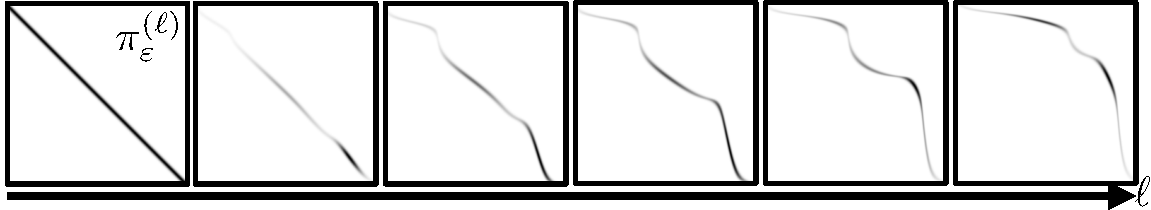
\includegraphics[width=.7\linewidth]{entropic/sinkhorn-convergence}
%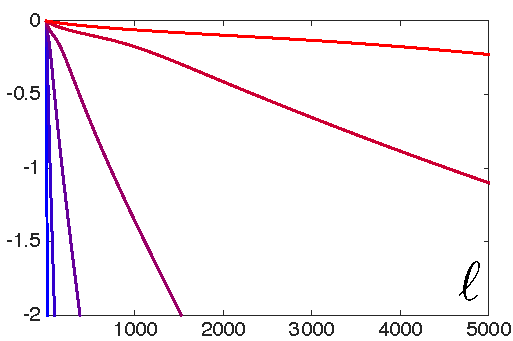
\includegraphics[width=.28\linewidth]{entropic/sinkhorn-rates}
%\caption{\label{fig-sinkhorn-convergence}
%Left: evolution of the coupling $\pi_\epsilon^\ell=\diag(\it{\UD})\K\diag(\it{\VD})$ computed at iteration $\ell$ of Sinkhorn's iterations, for 1-D densities.
%Right: impact of $\epsilon$ the convergence rate of Sinkhorn, as measured in term of marginal constraint violation $\log( \norm{\pi_\epsilon^\ell \ones_m - \b}_1 )$.
%}
%\end{figure}

A chief advantage, beside its simplicity, of Sinkhorn's algorithm is that the only computationnaly expensive step are matrix-vector multiplication by the Gibbs kernel, so that its complexity scales likes $Knm$ where $K$ is the number of Sinkhorn iteration, which can be kept polynomially in $1/\epsilon$ if one is interested in reaching an accuracy $\epsilon$ on the (unregularized) transportation cost. Note however that in many situation, one is not interested in reaching high accuracy, because targeted application success is often only remotely connected to the ability to solve an optimal transport problem (but rather only being able to compare in a geometrically faithful way distribution), so that $K$ is usually quite small.
%
This should be contrasted with interior point methods, which also operate by introducing a barrier function of the form $-\sum_i \log(\P_{i,j})$. These algorithm have typically a complexity of the order $O(n^6 \log(|\epsilon|))$ \todo{check}. 

The second crucial aspect of Sinkhorn is that matrix-vector multiplication streams extremely well on GPU. Even better, if one is interested in computing many OT problem with a fixed cost matrix $\C$, one can replace many matrix-vector multiplication by matrix-matrix multiplication, so that the computation gain is enormous. 


%%%%%%%%%%%%%%%%%%%%%%%%%%%%%%%%%%%%%%%%%%%%%%%%%%%%%%%%%%%%%%%%%%%%%%%%%%%
\subsection{Convergence}

%%%%
\paragraph{Convergence finite dimension via alternating projections.}

One has 
\eq{
	\dotp{\P}{\C} + \epsilon \KLD(\P|\a \otimes \b) = \epsilon \KLD(\P|\K) + \text{cst}, 
}
so that the unique solution $\P_\epsilon$ of~\eqref{eq-regularized-discr} is a projection onto $\CouplingsD(\a,\b)$ of the Gibbs kernel $\K$
\eql{\label{eq-kl-proj}
	\P_\epsilon = \Proj_{\CouplingsD(\a,\b)}^\KLD(\K) \eqdef \uargmin{\P \in \CouplingsD(\a,\b)} \KLD(\P|\K).
}

Denoting 
\eq{
	\Cc^1_\a \eqdef \enscond{\P}{\P\ones_m=\a}
	\qandq
	\Cc^2_\b \eqdef \enscond{\P}{\transp{\P}\ones_m=\b}
}
the rows and columns constraints, one has $\CouplingsD(\a,\b) = \Cc^1_\a \cap \Cc^2_\b$. One can use Bregman iterative projections~\cite{bregman1967relaxation}
\eql{\label{eq-kl-sinkh-proj}
	\itt{\P} \eqdef \Proj_{\Cc^1_\a}^{\KLD}(\it{\P})
	\qandq
	\ittt{\P} \eqdef \Proj_{\Cc^2_\b}^{\KLD}(\itt{\P}).
}
Since the sets $\Cc^1_\a$ and $\Cc^2_\b$ are affine, these iterations are known to converge to the solution of~\eqref{eq-kl-proj}, see~\cite{bregman1967relaxation}. 

The two projector are simple to compute since they corresponds to scaling respectively the rows and the columns
\eq{
	 \Proj_{\Cc^1_\a}^{\KLD}(\P) = \diag\pa{\frac{\a}{\P \ones_m}} \P
	 \qandq
	 \Proj_{\Cc^2_\b}^{\KLD}(\P) =  \P \diag\pa{\frac{\b}{\P^\top \ones_n}}.
}

These iterate are equivalent to Sinkhorn iterations~\eqref{eq-sinkhorn} since defining 
\eq{\label{eq-sink-matrix}\P^{(2\ell)} \eqdef \diag(\it{\uD}) \K \diag(\it{\vD}),}
one has
\begin{align*}
	\P^{(2\ell+1)} &\eqdef \diag(\itt{\uD}) \K \diag(\it{\vD}) \\
	\qandq
	\P^{(2\ell+2)} &\eqdef \diag(\itt{\uD}) \K \diag(\itt{\vD})
\end{align*}
In practice however one should prefer using~\eqref{eq-sinkhorn} which only requires manipulating scaling vectors and multiplication against a Gibbs kernel, which can often be accelerated (see below Remarks~\ref{rem-separable} and~\ref{rem-geod-heat}). 

Such a convergence analysis using Bregman projection is however of limited interested because it only works in finite dimension. For instance, the linear convergence speed one can obtain with these analyses (because the objective is strongly convex) will degrade with the dimension (and of course also with $\epsilon$). 
%
It is also possible to decay $\epsilon$ during the iterates to improve the speed and rely on multiscale strategies in low dimension.
 
% \todo{Remark on Bregman divergence, generalizatiton of projected gradient desc (mirror descent), etc.}



%%%%
\paragraph{Convergence for the Hilbert metric}

As initially explained by~\cite{franklin1989scaling}, the global convergence analysis of Sinkhorn is greatly simplified using Hilbert projective metric on $\RR_{+,*}^n$ (positive vectors), defined as
\eq{
	\foralls (\uD,\uD') \in (\RR_{+,*}^n)^2, \quad
	\Hilbert(\uD,\uD') \eqdef 
	\norm{\log(\uD)-\log(\vD)}_V
	% \log \umax{i,i'} \frac{ \uD_i \uD_{i'}' }{ \uD_{i'} \uD_{i}'  }.
}
where the variation semi-norm is
\eq{
	\norm{z}_V = \max(z)-\min(z).
}
One can show that $d_\Hh$ is a distance on the projective cone $\RR_{+,*}^n/\sim$, where $\uD \sim \uD'$ means that $\exists s>0, \uD=s\uD'$ (the vector are equal up to rescaling, hence the naming ``projective''), and that $(\RR_{+,*}^n/\sim,d_\Hh)$ is then a complete metric space.  
%
% This is a projective version of Hilbert's original distance on bounded open convex sets~\cite{hilbert1895gerade}.
%
It was introduced independently by~\cite{birkhoff1957extensions} and~\cite{samelson1957perron} to provide a quantitative proof of Perron-Frobenius theorem (convergence of iterations of positive matrices). Sinkhorn should be thought as a non-linear generalization of Perron-Frobenius. 

% , which, as explained in Remark~\ref{rem-local-conv} is linked to a local linearization of Sinkhorn's iterates. They proved the following fundamental theorem, which shows that a positive matrix is a strict contraction on the cone of positive vectors.

\begin{thm}\label{thm-birkoff}
	Let $\K \in \RR_{+,*}^{n \times m}$, then for $(\vD,\vD') \in (\RR_{+,*}^m)^2$
	\eq{
		\Hilbert(\K \vD,\K \vD') \leq \la(\K) \Hilbert(\vD,\vD')
		\text{ where }
		\choice{
			\la(\K) \eqdef \frac{ \sqrt{\eta(\K)}-1 }{ \sqrt{\eta(\K)}+1 } < 1 \\
			\eta(\K) \eqdef \umax{i,j,k,\ell} \frac{ \K_{i,k} \K_{j,\ell} }{ \K_{j,k} \K_{i,\ell} }.
		}
	}
\end{thm}

The following theorem, proved by~\cite{franklin1989scaling}, makes use of this Theorem~\ref{thm-birkoff} to show the linear convergence of Sinkhorn's iterations.

\begin{thm}
	One has $(\it{\uD},\it{\vD}) \rightarrow (\uD^\star,\vD^\star)$ and
	\eql{\label{eq-convlin-sinkh}
		\Hilbert(\it{\uD}, \uD^\star) = O(\la(\K)^{2\ell}), \quad
		\Hilbert(\it{\vD}, \vD^\star) = O(\la(\K)^{2\ell}).
	}
	One also has
	\eql{\label{eq-convsinkh-control}
		\Hilbert(\it{\uD}, \uD^\star) \leq \frac{\Hilbert( \it{\P}\ones_m,\a )}{1-\la(\K)} 
		\qandq
		\Hilbert(\it{\vD}, \vD^\star) \leq \frac{\Hilbert( \P^{(\ell),\top} \ones_n,\b )}{1-\la(\K)}, 
	}
	where we denoted $\it{\P} \eqdef \diag(\it{\uD}) \K \diag(\it{\vD})$. Lastly, one has
	\eql{\label{eq-convlin-sinkh-prim}
		\|\log(\it{\P}) - \log(\P^\star)\|_\infty \leq \Hilbert(\it{\uD}, \uD^\star) + \Hilbert(\it{\vD}, \vD^\star)
	}
	where $\P^\star$ is the unique solution of~\eqref{eq-regularized-discr}. 
\end{thm}

\begin{proof}
	One notice that for any $(\vD,\vD') \in (\RR_{+,*}^m)^2$, one has 
	\eq{	
		\Hilbert(\vD,\vD') = \Hilbert(\vD/\vD',\ones_m) = \Hilbert(\ones_m/\vD,\ones_m/\vD').
	}
	This shows that
	\begin{align*}
		\Hilbert(\itt{\uD},\uD^\star) &= \Hilbert\pa{ \frac{\a}{\K \it{\vD}}, \frac{\a}{\K \vD^\star} } 
		= \Hilbert( \K \it{\vD}, \K \vD^\star ) \leq \la(\K) \Hilbert( \it{\vD}, \vD^\star ).
	\end{align*}
	where we used Theorem~\ref{thm-birkoff}. This shows~\eqref{eq-convlin-sinkh}.  One also has, using the triangular inequality
	\begin{align*}
		\Hilbert(\it{\uD},\uD^\star) &\leq \Hilbert(\itt{\uD},\it{\uD}) + \Hilbert(\itt{\uD},\uD^\star) 
		\leq \Hilbert\pa{ \frac{\a}{\K \it{\vD}},\it{\uD} } + \la(\K) \Hilbert(\it{\uD},\uD^\star) \\
		&= \Hilbert\pa{ \a,\it{\uD} \odot  ( \K \it{\vD} ) } + \la(\K) \Hilbert(\it{\uD},\uD^\star), 
	\end{align*}
	which gives the first part of~\eqref{eq-convsinkh-control} since 
	$\it{\uD} \odot  ( \K \it{\vD} ) = \it{\P}\ones_m$ (the second one being similar).
	%
	The proof of~\eqref{eq-convlin-sinkh-prim} follows from~\cite[Lemma 3]{franklin1989scaling}
\end{proof}
 
The bound~\eqref{eq-convsinkh-control} shows that some error measures on the marginal constraints violation, for instance $\| \it{\P} \ones_m - \a \|_1$ and $\|\transp{\it{\P}} \ones_n - \b \|_1$, are useful stopping criteria to monitor the convergence. 
%
This theorem shows that Sinkhorn algorithm converges linearly, but the rates becomes exponentially bad as $\epsilon \rightarrow 0$, since it scales like $e^{-1/\epsilon}$. In practice, one eventually observes a linear rate after enough iteration, because the local linear rate is much better, usually of the order $1-\epsilon$. 

% Figure~\ref{fig-sinkhorn-convergence}, bottom row, highlights this linear rate on the constraint violation, and shows how this rate degrades as $\epsilon\rightarrow 0$. 
%
% These results are proved in~\cite{franklin1989scaling} and are tightly connected to nonlinear Perron-Frobenius Theory~\cite{lemmens2012nonlinear}. Perron-Frobenius theory corresponds to the linearization of the iterations, see~\eqref{eq-linearized-sinkh}. This convergence analysis is extended in~\cite{linial1998deterministic}, who shows that each iteration of Sinkhorn increases the permanent of the scaled coupling matrix. 

